%\documentclass[referee]{svjour3} % insert '[draft]' option to show overfull boxes
\documentclass[onecolumn]{svjour3} % insert '[draft]' option to show overfull boxes

 \title{A Graph Theoretic Approach to Problem Formulation for Multidisciplinary Design Optimization}
        
\author{
  David J. Pate, %
  Justin Gray, %
  Brian J. German 
 }

 \institute { Justin Gray 
	\at NASA Glenn Research Center, Mail Stop 5-11, 21000 
		Brookpark Rd Clevland OH 44135 %
	\and David J. Pate 
	\at Graduate Research Assistant, Georgia Institute of Technology, 270 Ferst Drive, Atlanta, GA, 30332, U.S.A.
	\and Brian German 
	\at Assistant Professor, Georgia Institute of Technology, 270 Ferst Drive, Atlanta, GA, 30332, U.S.A.}
 
\journalname{Structrual and Multidisciplinary Optimization}

%\usepackage{setspace}
%\doublespace

\usepackage{graphicx}
\usepackage{wrapfig}
\usepackage{caption} 
\usepackage{amsmath}
\usepackage{amssymb}
\usepackage{amsfonts}
\usepackage{lscape}
\usepackage{hyperref}
\usepackage{appendix}
\usepackage[section]{placeins}
\usepackage[retainorgcmds]{IEEEtrantools}
\usepackage{subfigure}
\usepackage{comment}
\usepackage{booktabs}

\captionsetup[figure]{margin=5pt,font=small,labelfont=bf,textfont=bf,justification=justified,}
%\captionsetup[wrapfigure]{margin=5pt,font=small,labelfont=bf,justification=justified,singlelinecheck=off}
\captionsetup[table]{margin=5pt,font=small,labelfont=bf,textfont=bf,justification=justified,position=top}

\bibliographystyle{aiaa}

\usepackage{lettrine}
\usepackage{verbatim}

\newcommand{\txt}{\textrm}

%\usepackage{hyperref} %allows for the creation of actual text links
\begin{document}

\maketitle
 
\begin{abstract}
The formulation of multidisciplinary design, analysis, and optimization (MDAO) problems has become increasingly complex as the number of analysis tools and design variables included in typical studies has grown.  This growth in the scale and scope of MDAO problems has been motivated by the need to incorporate additional design disciplines and to expand the parametric design space to enable the exploration of unconventional design concepts.  In this context, given a large set of disciplinary analysis tools, the problem of determining a feasible data flow between tools to produce a specified set of system-level outputs is combinatorically challenging.   The difficulty is compounded in multi-fidelity problems, which are of increasing interest to the MDAO community.  In this paper, we propose an approach for addressing this problem based on the formalism of graph theory.  The approach begins by constructing the maximal connectivity graph (MCG) describing all possible interconnections between a set of analysis tools. Graph operations are then conducted to reduce the MCG to a fundamental problem graph (FPG) that describes the connectivity of analysis tools needed to solve a specified system-level design problem. The FPG does not predispose a particular solution procedure; any relevant MDO solution architecture could be selected to implement the optimization.  The approach is applied to an example problem to formulate an FPG for a commercial aircraft MDAO study.
\end{abstract}

\section*{Nomenclature}

\begin{tabular}{l l} 
    AAO      & All-At- \\
    MDAO     & Multidisciplinary Design Analysis and \\ & Optimization \\
    FPF      & Fundamental Problem Formulation \\
\end{tabular}

\section{Introduction}
    
    As the size and complexity of engineering systems grow, the time and expense for setting up 
    analysis models grow with them. Multidisciplinary Design Analysis and Optimization (MDAO)
    frameworks such as OpenMDAO\cite{Gray2012} and ModelCenter have enabled a new level of analysis tool integration 
    and paved the way for models with more analyses and increasing numbers of interdisciplinary couplings. That 
    new capability has created a new challenge since configuring a model with the larger nubmer of analyses, associated inputs and outputs
    can be very difficult. Even for models with 10's of analyses, there could be hundreds of variables that need to be managed. 
    It is not hard to imagine that the task of combining all the analyses into a consistent system model capable of solving a relevant 
    engineering design problem could easily become much more costly than createing the discipline analyses themselves. Thus, for a large system
    as the couplings between the disciplines begin to dominate the design space, the couplings between the analyses begin to dominate 
    the job of setting up the model. 
    
    When building a model, coupling represents the reciprical flow of information between two analyses. 
    We propose the use of graph-based syntax to describe the flow of information from inputs, 
    through analyses, to outputs. If you allow for any free inputs to become design
    variables and some set of the outputs to become design objectives and constraints, then the graph 
    represents the problem formulation for a given design effort. 
    The graph-based syntax presented has application in all phases of the design process. 
    It can be used early on, to help construct a valid problem formulation from the set of available analysis tools. 
    It also provides a consistent structure to describe problem formulation that provides a foundation to apply
    algorithmic methods for selecting and then implementing effective solution strategies inside an MDAO framework. 

    We've already identifed that a problem formulation graph should include design variables, analysis tools and their 
    associated inputs and outputs, and objectives and constraints. Notably absent from that list are any kind of 
    solvers, optimizers, or other iterative solution finding tools. At its most fundamental state, a problem formulation 
    includes only information about what is being sought after in a design or what the
    goals of a given problem are. It need not contain any information about solution paths or strategies to reach those goals. 
    While solution information can be represented with the graph syntax presented here, a unique aspect of this syntax is that 
    such information always remains seperable from the underlying problem formulation. In other words, a given a graph representing 
    a specific solution strategy for a specific problem formulation, it is possible to remove the solution information from the 
    graph and reclaim the more basic problem formulation. 


\section{Specific vs Fundamental Problem Formulation }

    The Fundamental Problem Formulation (FPF) for any given problem will be constant regardless 
    of which MDAO framework, optimization algorithm, iterative solver, or solution strategy
    is used to solve the problem. For example, consider the following notional problem: 

    \begin{align}
        given & \ \ A: {x,y} \rightarrow {m,z} \notag
        \\      & \ \ B: {x,z} \rightarrow {y^t} \notag
        \\min. &\ \ f(m) \notag
        \\w.r.t. & \ \ x,y,z \notag
        \\s.t. & \ \ g(y^t,y) = 0
        \label{eqn:simple}
    \end{align}

    $A$ and $B$ represent analysis tools, and $f$ and $g$ are the objective and constraint functions respectively. 
    Equation \ref{eqn:simple} makes an inherent assumption about the solution strategy for the problem. 
    Analysis $A$ outputs $z$, which is an input to $B$. Hence, $A$ should be run before $B$ with 
    with $y$ being iterated on to convergence with $y^t$. However, a slightly different formulation is 
    equally valid and still represents the exact same problem: 

    \begin{align}
        given & \ \ B: {x,z} \rightarrow {y} \notag
        \\      & \ \ A: {x,y} \rightarrow {m,z^t} \notag
        \\min. &\ \ f(m) \notag
        \\w.r.t. & \ \ x,y,z \notag
        \\s.t. & \ \ g(z^t,z) = 0
        \label{eqn:simple2}
    \end{align}

    Equation \ref{eqn:simple2} differs only slightly from Eq. \ref{eqn:simple}. $A$ is now dependent on the output of $B$, 
    and $z$ will be iterated on to convergence with $z^t$. Now the problem can be solved by running $B$ first and then $A$.
    Since the formulations in Eqs. \ref{eqn:simple} and \ref{eqn:simple2} both describe the same problem and neither can be the
    FPF. They are both specific versions of the same more fundamental description of 
    the problem that is common between them. We present the FPF as follows: 

    \begin{align}
        given & \ \ A: {x,y} \rightarrow {m,z^t} \notag
        \\      & \ \ B: {x,z} \rightarrow {y^t} \notag
        \\min. &\ \ f(m) \notag
        \\w.r.t. & \ \ x,y,z \notag
        \\s.t. & \ \ g1(z^t,z) = 0 \notag
        \\     & \ \ g2(y^t,y) = 0
        \label{eqn:simple_fpf}
    \end{align}

    The FPF in Eq. \ref{eqn:simple_fpf} differs from both Eq. \ref{eqn:simple} and Eq. \ref{eqn:simple2} because it has 
    two constraints which both must be met. The presence of both of these constraints fully decouples the problem so that 
    either $A$ or $B$ could be run first or both could be run simultaneously. By removing either constraint and replacing 
    it with a direct dependence between the two analyses you could regain the earlier two problem formulations. Alexandrov
    and Lewis demonstrated the value of a more modular approach to problem formulation because it enables one to transition between different 
    MDAO solution strategies depending on the specifics of the problem\cite{Alex2000}.


\section{Existing Graph--Based Problem Formulation Syntax}

    As shown above, the mathematical language for specifying problem formulations is very general and can be used both for 
    fundamental and specific problem formulations. Tedford and Martins used the above mathematical syntax to specify the 
    FPF for a set of test problems and also to describe specific formulations for solving them with a 
    number of optimization architectures\cite{Tedford2009}. Their work demonstrates clearly how multiple specific 
    problem formulations can all relate back to a common FPF. The challenge with using this 
    traditional mathematical syntax is that it is not easily manipulated or analyzed. 
    A number of graph-based methods have been used successfully to translate the 
    mathematical syntax into a more useful computational form. 
    
    Steward's Design Structure Matrix (DSM) is a square adjacency matrix which captures the relationship between analysis tools where off 
    diagonal elements of the matrix indicate coupling\cite{Steward1981}. Since a DSM describes a square adjacency matrix, 
    it can be represented in an equivalent directed graph where nodes represent analysis tools and 
    edges represent information dependence between those tools. The ordering of elements in a DSM can be used to indicate 
    execution order.  For more complex problems, choosing the proper order to run analysis tools is a non-trival task. 
    Rogers et. al developed DeMAID to manipulate a DSM to find an ordering for analysis tools that 
    reduces the cost of solving highly coupled systems\cite{Rogers1996}. This re-ordering is done through 
    row operations on the DSM matrix and yields multiple specific problem 
    formulations which all solve the same FPF. In other words, manipulation of the DSM does not fundamentally alter
    the problem formulation, which makes DSM an excellent foundation for specifying the FPF itself. 
    
    Despite it's attractive properties, a DSM by itself is insufficient to describe complete problem formulations. 
    Traditional DSM only captures information about data dependency between analyses. 
    Objective and constraint information is missing from the description of the problem. 
    An alternative matrix-based syntax, called a Functional Dependency Table (FDT), was proposed by Wagner and Papalambros. 
    FDT represents the relationship between functions, including objectives and constraints, and specific variables that affect 
    them\cite{Wagner1993}. Similar to DSM, FDT also describes an adjacency matrix of a graph. Unlike the DSM graph, 
    however, the graph is undirected and nodes can represent analysis tools, objectives, 
    or constraints. Edges between nodes represent a dependence on the same 
    variable. Michelena and Papalambros made use of the FDT to solve a graph partitioning problem that yielded 
    more efficient optimization problem decompositions\cite{Michelena1997}. While FDT succeeds at capturing the 
    information about objectives and constraints, it can not capture the coupled data dependency that DSM captures. For instance, 
    we know from the FPF in Eq. \ref{eqn:simple_fpf} that the objective, $f$, is dependent on the 
    output, $m$, of analysis $A$. You could not determine that from the FDT in Fig. \ref{fig:FDT_simple} alone. This missing 
    information means that, while FDT is very useful for partitioning problems, it is also not sufficient to contain a 
    complete problem formulation. 

    \begin{figure}
        \begin{center}
        \begin{tabular}{|c|c|c|c|c|c|c|}
            \hline
                 & $x$ & $y$ & $y^t$ & $z$ & $z^t$ & m \\ \hline
            $A$  & 1  & 1    &       &     &       &   \\ \hline
            $B$  & 1  &      &       & 1   &       &   \\ \hline
            $f$  &    &      &       &     &       & 1 \\ \hline
            $g1$ &    &      &       & 1   & 1     &   \\ \hline
            $g2$ &    & 1    & 1     &     &       &   \\
            \hline
        \end{tabular}
        \caption{Functional Dependency Table (FDT) for Eq. \ref{eqn:simple_fpf} \label{fig:FDT_simple}}
        \end{center}
    \end{figure}

    Lamb and Martins included objectives and constraint functions as nodes in an Extended 
    DSM (XDSM) in order to capture a more complete description of solution strategies for MDAO problems\cite{Lambe2012}. 
    XDSM retains the square adjacency matrix form from DSM, but by adding in the 
    new elements they partially combined a traditional DSM with an FDT. 
    This allows XDSM to represent data dependency between multiple analysis tools as well as between analysis tools and
    objective/constraint functions. With the additional information included in an 
    XDSM, Lu and Martins applied both ordering and partitioning 
    algorithms on an MDAO test problem named the Scalable Problem \cite{Lu2012}. 

    \begin{figure}
        \begin{center}
        \includegraphics[height=.25\textheight]{XDSM/simple}
        \caption{XDSM for Eq. \ref{eqn:simple}, with a gauss-siedel iteration and MDF solution architecture. \label{fig:XDSM_simple}}
        \end{center}
    \end{figure}

    Although XDSM captures part of the functional aspects of FDT, it leaves out the variables themselves.  
    As a result, all variable information is aggregated 
    so that for the problem from Eq. \ref{eqn:simple_fpf} you can say that $A$ 
    depends on $B$ or vice versa, but you can't identify which 
    individual variables are interacting in the dependency cycle. 
    Without the detailed variable information, you can't construct the compatibility 
    constraints necessary to implement the problem. Additionally, XDSM 
    requires the use of solver and optimizer blocks to represent 
    the relationship between design variables and objectives/constraints. 
    By introducing solver or optimizer blocks XDSM automatically provides
    some kind of solution strategy. The XDSM for Eq. \ref{eqn:simple} is 
    given in Figure \ref{fig:XDSM_simple}. This diagram is shown with an 
    assumed gauss-siedel iteration scheme and a MDF solution architecture. 
    Hence XDSM is too specific for use with a fundamental problem formulation. 

    Of the three methods, XDSM comes the closest to fully describing a problem formulation. 
    Thought it does not contain specific variable information, this could be easily added back in
    simply by putting the variables back into the graph and drawing the apprpriat connections
    between them and the relevant analysis nodes. However, it's dependence on 
    solution strategy specifics to represent couplings can not be removed without 
    stripping it of the useful information contained in an FDT. In the following sections
    we describe a new graph syntax that retains the features of XDSM, without the dependence on 
    solution strategy (although it does allow for that information to be present). Thus 
    the new syntax allows for the compelete specification of an FPF. 
\newcommand{\st}{ \ | \ }

\section{Requirements for New Graph Syntax}
  \label{s:requirements}
  The ultimate goal of the new graph--based syntax presented here is to be able to 
  fully describe the general structure of an MDAO problem independently of any solution information, 
  while still being able to accomodate the more specific case when a solution 
  strategy is applied. In order to achieve that goal 
  the graph needs to accomodate a number of constructs of MDAO problems: 
  \begin{itemize}
    \item Analysis tools and connections between them
    \item Design variables, objectives, and constraints
    \item Local and global properties
    \item Coupling between analyses
    \item Multi-fidelity analyses
  \end{itemize}

  Beyond those basic constructs, there are also three phases of a design process that 
  all need to be representable with the new syntax. Firstly there is the initial problem definition
  phase where the specific analysis tools and design goals are identified. At the end of this phase, 
  a single formal problem formulation is selected specifying design variables, constraints, objectives, 
  analysis tools, etc. Lastly some specific procedure for solving the problem is selected, for example 
  picking an MDAO optimization architecture. Using the proposed graph syntax, each of these phases 
  can be represented with the following three graphs:
  \begin{itemize}
    \item Maximal Connectivity Graph (MCG)
    \item Fundamental Problem Graph (FPG)
    \item Problem Solution Graph (SPG)
  \end{itemize}

  The \emph{maximal connectivity graph} represents the first phase with all 
  analysis codes being considered and all possible connections between them also present. The second graph 
  is the \emph{fundamental problem graph}, which is the smallest possible graph 
  that still fully defines a given problem formulation. Finally, a \emph{specific problem formulation} 
  may be represented by including additional edges and nodes to represent the 
  solution strategy being employed to solve the problem. 

  The relationship between these three graphs is depicted in Figs.~\ref{f:tree} and \ref{f:hourglass}. 
  The tree diagram demonstrates the fact that it is generally possible to obtain 
  multiple FPGs from a single maximal connectivity graph. This  may correspond to 
  different down--selections of analysis codes, different connections between them, 
  or both. Each down--selection shrinks the number of possible FPGs that could be reached 
  until only one is remaining. Then, from a single FPG, different PSGs may be obtained by implementing 
  different solution strategies. If you consider the size of a graph to be the sum of all of its
  edges and nodes then the hourglass shape in Fig. \ref{f:hourglass} illustrates how
  the MCG gets reduced to a single FPG, then multiple possible PSGs exist to solve the problem.
  In other words the FPG is obtained from the MCG by removing nodes and edges, 
  and the PSG is obtained from the FPG by adding nodes and edges.

  \begin{figure}[htb!]
    \centering
    \subfigure[number of possible graphs]{
    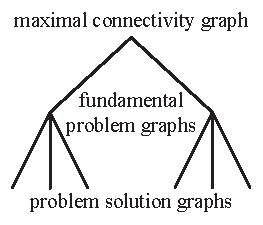
\includegraphics[width=2.0in]{images/tree}
    \label{f:tree}
    }
    \subfigure[graph size]{
    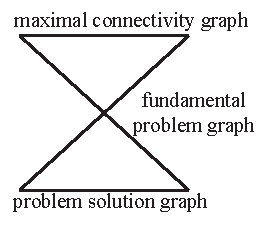
\includegraphics[width=2.0in]{images/hourglass}
    \label{f:hourglass}
    }
  \caption{The relationship between the MCG, FPG, and PSG.}
  \end{figure}

\section{Syntax Definition}
  \label{s:syntax definition}
  In this section we present the necessary graph theory fundamentals to 
  construct the graphs discussed above. 
  The notation used in this work is adapted from Diestel \cite{Diestel2010}. 
  A \emph{graph} is a pair $G = (V,E)$ of sets such that $E \subseteq V \times V$, 
  which means that the elements of $E$ are 2--element subsets of $V$. The set $V$ 
  contains the \emph{vertices} or \emph{nodes} and the set $E$ contains the \emph{edges}.
  For a \emph{directed graph*} (or \emph{digraph}) we construct $E$ as a set of ordered pairs instead 
  of a set of sets. Each ordered pair represents an edge starting at the node 
  indicated by the first entry and directed to the node indicated by the second 
  entry. Edge $e$ = $(x,y)$ may be referred to simply as $xy$. For node $v \in V$ 
  the edges directed out are given by $E(v)$ and the edges directed into $v$ are given 
  by $E^{-1}(v)$; $E(E(v))$ is denoted as $E^2(v)$, and likewise for additional levels. 
  If $E$ is not a one--to--one mapping, $E(v)$ may be the empty set, a single node, or a set of nodes.
  \begin{figure}[htb!]
    \begin{center}
    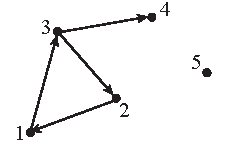
\includegraphics[width=1.5in]{images/example_directed_graph}
    \end{center}
    \vspace{-20pt}
  \caption{Example directed graph.}
  \label{f:example directed graph}
  \end{figure}
  As an example, for the directed graph shown in Fig.~\ref{f:example directed graph} we have
  \begin{IEEEeqnarray*}{rCl}
  V & = & \{1,2,3,4,5\}, \\
  E & = & \big\{(1,2),(3,2),(1,3),(3,4)\big\}.
  \end{IEEEeqnarray*}

  A \emph{path} $P=(V,E)$ from $x_0$ to $x_k$ in graph $G$ is a subgraph of $G$ with $V = \{x_0,x_1,\ldots,x_k\}$ and $E = \{(x_0,x_1),(x_1,x_2),\ldots,(x_{k-1},x_k)\}$.
  A \emph{reverse path} $P_R$ in graph $G$ is a path on $R$, where $R$ is the reverse graph of $G$ obtained by switching the orientation of every edge.


  %does this belong in the analysis block section???? 
  Let $I$ be a nonempty set of counting numbers such that for each $i \in I$ there is a corresponding set $A_i$. 
  The set of sets $\mathcal A = \{A_i \st i \in I\}$ is called an indexed family of sets with index $i$ and 
  indexing set $I$\cite{smith2006}. 
  The union over this family of sets can be described in a few different ways:
  \begin{equation}
  \bigcup_{i \in I} A_i = \bigcup_{A \in \mathcal A} A = \{x \st x \in A \txt{ for some } A \in \mathcal A\}.
  \end{equation}

  Lastly, the cardinality of a set $B$ is the number of elements in $B$ and is denoted as $|B|$.

\subsection{Node and Edge Types}
  \label{ss:types}
  We now define different types of nodes and edges with specific properties to compose graphs used to represent an MDAO problem. 
  There are three node types:  
  \begin{description}
    \item[variable:] represents scalar or array data
    \item[model:] responsible for mapping inputs to outputs
    \item[driver:] control logic capable of managing iteration
  \end{description}

  In addition to the three node types, there are two edge types: 

  \begin{description}
  \item[connection edge:] Exchange of information between two nodes. These edges 
  can either be fixed (can not be removed from graph) or free (can be removed). 
  \item [driven edge:] Passing of information from a driver node to a 
    variable node. A single variable node can have many incomming driven edges. These edges are 
    free and can be added or removed from the graph. 
  \end{description}

  [[Insert legend for node and edge types]]

  In Alexandrov and Lewis's REMS syntax only two node types were present, variable 
  and function, and only one edge type\cite{alexandrov2004}. We've chosen to rename the ``function'' node 
  type to ``model'' to be more consistent with modern MDAO frameworks. The present work 
  adds one more node types and one more edge type to the syntax to allow descriptive
  graphs for all three phases of the design process. In addition, we introduce the 
  concept of fixed vs. free connection edges to represent the
  static relationship between variable and model nodes from a single analysis, 
  vs the flexible relationship between variables from different analyses. 

\subsection{Rules for Nodes and Edges}
  \label{ss:rules}
  There are specific rules for the usage of these nodes and edges.
  The driver node and the driven edge are only allowed to be present in PSGs. All 
  other node and edge types can be present in any of the three graphs, subject to these restrictions: 
  \begin{enumerate}
  \item A model node can only have one edge directed to or from another model node.
  \item A model node can only have fixed connection edges directed in or out.
  \item A model node must have at least one edge directed in and at least one edge 
    directed out.
  \item If a variable node has an outgoing edge to a model node then it may not have 
    any other outgoing edges.
  \end{enumerate}

\subsection{indegree and outdegree}
  \label{s:indegree-outdegree}
  The \emph{indegree} of a node is the number of connection edges directed in and 
  is denoted as $\txt{deg}^-(v)$, and the \emph{outdegree} 
  is the number of connection edges directed out and it is denoted as $\txt{deg}^+(v)$.
  The degree of a given node is only a function of the connection edges 
  attached to it. The number of driven edges is not relevant since any number 
  of drivers could be involved, at different parts of an solution process. For 
  example in a sequential optimization where a global optimizer is first applied
  and a gradient based one is applied second, design variables would have incomming 
  driven edges from both optimizers but this would not affect the indegree of those
  variable nodes. 

  Specifially for variable nodes we also define the \emph{upper indegree limit} 

  \begin{equation}
  \txt{deg}_u^-(v):V \to \mathbb{N}
  \end{equation} 
  and the \emph{lower indegree limit} as
  \begin{equation}
  \txt{deg}_l^-(v):V \to \mathbb{N}.
  \end{equation}
  These user-specified limits govern the number of connection edges that may 
  be directed into a variable node for a valid graph. Consider a variable 
  node $v$ with $\txt{deg}_u^-(v) = \txt{deg}_l^-(v) = 1$. In this case, $v$ 
  must have exactly one incomming explicit edge or the graph is invalid. 
  Two possiblities exist for voilating these limit conditions: 

  \begin{description}
    \item[hole: ] The number of incomming edges is less than the lower indegree limit:
      \begin{equation} \txt{deg}^-(v) < \txt{deg}_l^-(v) \label{e:hole} \end{equation}
      This represents a lack of information being supplied to the node.
    \item[collision: ] The number of incomming edges is greater than $ \txt{deg}_u^-(v)$. 
      \begin{equation} \txt{deg}^-(v) > \txt{deg}_u^-(v) \label{e:collision}\end{equation}
  \end{description} 

  The presence of holes and collisions in a graph represent issues that will give
  rise to an invalid problem formulation. An algorithm for detecting and 
  managing these violations if proposed in Sec.~\ref{s:building graphs}.\ref{ss:obtaining FPG}.

\section{Graph Representation of MDAO Constructs}
\label{s:graph representation}
In this section we will make use of the Sellar problem, described in 
Eqn. \ref{eqn:simple_fpf}. The graph representation of the Sellar problem, 
using the new stynax, is presented in Fig. \ref{f:sellar_graph_full}. Throughout
the rest of this section, different sub-graphs or slight modifications of 
the full graph will be used to demonstrate the important MDAO constructs within
this graph syntax.

\begin{figure}[htb!]
    \begin{center}
    \includegraphics[width=4in]{images/sellar_graph_full}
    \end{center}
    \vspace{-10pt}
\caption{Graph of the Sellar problem formulation}
\label{f:sellar_graph_full}
\end{figure}

\subsection{Analysis Blocks and Connections}
\label{ss:analysis blocks and connections}
Analysis tools take in a number input variables and then perform some work to calculate 
the values for their respective outputs. In an MDAO graph, this process is 
represented by a group of nodes and edges called an \emph{analysis block}, 
shown in Fig. \ref{f:analysis block}. Within an analysis block each variable 
node represents a single input or output and is connected 
to a single model node via a fixed edge. Note that in Fig.~\ref{f:analysis block}, 
the analysis block contains two model nodes, with a single edge connecting them. 
This edge represents the necessary calculations to map given inputs 
to proper output values. If constructing a weighted graph, the weight calculation edge 
provides the opportunity to computational cost. However, it is also allowed to 
skip this edge and have both incomming and outgoing edges to variables through a 
single model node for a given analysis block. Although analysis blocks are 
comprised of multiple nodes and edges, since all the edges within them are 
fixed, they become fixed sub-graphs within a graph. In this way, they cannot be 
altered but they can be removed as a group.

\begin{figure}[htb!]
    \begin{center}
    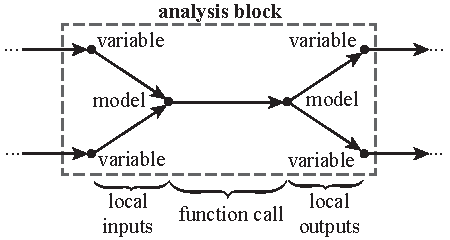
\includegraphics[width=4in]{images/analysis_block}
    \end{center}
    \vspace{-10pt}
\caption{Example analysis block. The each node type and edge type is labeled in italics and annotated parenthetically.}
\label{f:analysis block}
\end{figure}

Variable nodes in an analysis block can be distinguished as either an input or 
an output by the manner in which they are connected. As shown in Fig.~\ref{f:analysis block}, 
inputs are any variable nodes that have an outgoing edge into a model 
node. Conversely, outputs are any variable nodes that have an incoming edge from a model node. 

MDAO problems require that information be passed between sets of analyses. When 
information from the output of one analysis block is passed, or connected, to the 
input of another analysis block, a new connection edge is added connecting the two 
variable nodes involved in the exchange. These connection edges are free, unlike the edges 
within an analysis block, can be added or removed depending on the needs
of a given design problem. In other words, free connection edges are created by 
engineers linking the output of one tool to the input of another one. Note that 
it is allowed for a single output to have outgoing connection edges to multiple 
downstream inputs. 

\subsection{Design Variables}
For the Sellar problem, there are three design variables, $x_1^*$, $z_1^*$, and $z_2^*$. In Fig. 
\ref{f:sellar_graph_full}, these are the only three holes (nodes without out 
incomming edges) in the graph. 

\begin{figure}[htb!]
  \begin{center}
  [NOTE: Re-work this one to match $D_2$ from Sellar]
    \includegraphics[width=.6\textwidth]{images/design_vars_graph}
  \end{center}
  \caption{Notional graph with two potential design variables \label{f:designvars}}
\end{figure}

More formally stated, given a MCG with the $\txt{deg}_l^-(v)=1$ for all nodes, 
there will likely be a set of holes preventing a valid FPG from being obtained. 
Each hole represents a node that could potentially become a design variable. 
It is up to the designer to examine each and decide if it is appropriate to 
consider it a design variable, in which case the designer shall set the lower 
indegree limit to be zero. However, some variable holes may not actually be 
suitable as a design variable. For instance, if an aircraft mission analysis 
code requires a drag input which ends up being a hole then it's likely best to 
leave$\txt{deg}_l^-(v)=1$ and find a new analysis code to fill the hole in graph. 

So a design variable is defined as any variable node with $\txt{deg}_l^-(v)=0$. 
This, by definition, means that design variables are not holes in the graph, since 
they have not violated their lower indegree limit. Regardless, 
when working with a MCG or FPG, only connection edges are allowed, so a design 
variable in either graph will be a variable with no incomming edges edges. For a valid PSG 
any design variable node would have at least one, but possibly multiple, incomming 
driven edges from one or more driver nodes. 

\subsection{Objectives, and Constraints}
\label{ss:objectives and constraints}
Like design variables, objectives and constraints are also constructs that need 
to be identified when setting up a given design problem. In the case of 
objective functions single output values could be selected, but commonly multiple 
values are assembeled together via simple algebraic expressions to form a composite 
objective function. (e.g. The objective function from Eqn. \ref{eqn:simple_fpf} is
$x_1^2+z_2+y_1+e^{-y_2}$). Constraints are always given in the 
form of either an inequality or an equality. (e.g. a constraint from Eqn. 
\ref{eqn:simple_fpf} is $\frac{y_1}{3.16}-1\geq0$.) By convention, 
constraints are usually given such that some expression will be less than or equal 
to zero, so any positive value would violate the constraint. For both objective 
and constraints, these simple expressions take some inputs and map them to an
output value of significance to the overall design problem. 

These operations, though very simple, are effectively the same kind of task 
performed by an analysis block. A constraint or objective function can therfore 
be represented as another analysis block on the graph, with it's own input and 
output variable nodes. Although fundamentally no different than an analysis block, 
for clarity and convience it is useful to distinguish between regular analysis 
blocks and those that arise from the addition of objectives or constraints to 
the graph. Therefore, we define an \emph{expression block}, as the collection of variable and model 
nodes related to a given objective or constraint function. Fig. \ref{f:obj-cons}
highlights the objective and constraint blocks from the Sellar problem. 



\begin{figure}[htb!]
  \begin{center}
    \includegraphics[width=.6\textwidth]{images/obj_const_graph}
  \end{center}
  \caption{Notional graph with and objective and constraint nodes \label{f:obj-cons}}
\end{figure}


\subsection{Local vs Global Nodes}

  A simple definition of a global node is any node that involves information 
  from more than one analysis block. Likewise, a local node is any node 
  that involves information from only a single analysis block. As stated before, variable 
  nodes with fixed edges directed to model nodes (as part of an analysis block) are inherently local 
  and similarly model nodes are also local. Global variables are a part of many 
  MDAO problems and must be representable in the graph. Follwoing our simple definition
  any variable node that had multiple incomming or outgoing edges, would be global. 
  In Fig. \ref{f:sellar_graph_full} the variable nodes for $x_1^*$, $z_1^*$, and $z_2^*$ 
  have multiple outgoing edges and would be considered global. 

  Note that the variable $x_1$ from the Sellar problem is usually refered to as 
  a local variable, which is contradicted by the given graph. This discrepancy 
  arises from the explicit treatment of objectives and constraints as separate 
  expression blocks. Normally in the Sellar problem $x_1$ is considered a local 
  variable because it only directly affects analysis block $D_1$. By forcing
  the expansion of $F$ into an expression block with its own inputs, then $F$ 
  gets it's own copy of the $x_1$ variable. This necessitates the creation 
  of the global $x_1^*$ node in the graph with two outgoing edges to link the 
  two $x_1$ inputs nodes in the different blocks. Interestingly, using this 
  definition, where $x_1^*$ is a global variable fits nicely within 
  the structure of Braun's Colaborative Optimization (CO) archtiecture \cite{braun1996thesis}. 
  The rules of setting up a problem with CO require that each discipline be 
  given an independent local copy of all global variables. All local 
  variables are retained uniquely within their respective disciplines, except 
  when a local design variable shows up explicitely in the objective 
  or global constraint. In that case a global variable is created, and the discipline again 
  gets an independent local copy of it. Given our definition of global vs local
  variable nodes, no such exception for local variables in global expressions is 
  necessary. When you include a given variable in an expression block, it becomes 
  global by definition and should be treated as such in CO. 

  Analysis and expression blocks can also have a locality defined for the set of 
  nodes and edges within the block. Their locality is determined by the 
  incomming and outgoing edges from the block as a whole. Fig. 
  \ref{f:sellar_graph_full} has expression blocks for each constraint, 
  $G_1$ and $G_2$. Both constraints are local to their respective analysis 
  blocks. But the expression block for $F$ has incomming edges from $D_1$ and 
  $D_2$, so it would considered global. 

  Simply stating that any node or block with incomming or outgoing edges
  from more than one other node or block is global works glosses over a more 
  subtle aspect of some MDAO problems. The locality of any node in a graph is 
  a relative property. For instance, a single node might have outgoing edges 
  to two separate analysis blocks, $A$ and $B$, but none to a third, $C$. Then 
  you could say that this node was global with respect to $A$ and $B$ separately, but local 
  to the group $A,B$. This situation produces a natural 
  hierarchy in a graph, where you could form increasingly smaller groups as you 
  segment problem into finer localities. 

  When solving a problem using a heirarchical decomposition approach, 
  there are various techniques for partitioning that are effective in different 
  scenarios \cite{krishnamachari1997optimal,michelena1997hypergraph,sobieszczanski1997,Perez2004,allison2009optimal}. 
  Tosserams et al proposed a language based syntax for describing the partitioning of problems, named $\Psi$
  \cite{tosserams2010specification}. $\Psi$ provides an opposing perspective to 
  this work, where they compose hierarchies from the bottom up, into larger and 
  larger groups. However, $\Psi$ provides a compiler that can produce a standard 
  problem representation of the assembled problem, and a number of example converters
  from that standard representation to application specific formats. 

  [[Could probably build this and include it in appendix]] 


\subsection{Coupling Between Analyses}

  Coupling exists in a design problem when a set of two or more analyses each depend on the
  others outputs. In the Sellar problem from Eqn \ref{eqn:simple_fpf} the two 
  coupling constraints, $H_1$ and $H_2$ provide a reciprical dependence between 
  $D_1$ and $D_2$. In a graph, these constraints show up as connection edges between 
  the outputs of each analysis block. The relevant connection edges are highlighted in 
  Fig. \ref{f:coupling}, where they form a cycle. Cycles of connection edges are the characteristic 
  structure that represents coupling. 

  \begin{figure}
      \begin{center}
      %\includegraphics[height=.25\textheight]{}
      [INSERT GRAPH HERE]
      \caption{Graph of a notional problem with simple coupling \label{f:coupling}}
      \end{center}
  \end{figure}

  It is important to note that the coupling cycles do not contain 
  any driver nodes. Solver, optimizer, or other iterative process is 
  invovled in the coupling definition--though one will be necessary for a valid 
  PSG. Additionally, a coupling cycle has no inherant start or end. It would be
  valid to pick any node in the cycle as a starting point, and proceed around the
  loop untill you get back to your starting point. For the Sellar Problem, picking 
  $D_1$ as the starting point would yeild a problem as given in 
  Eqn.~\ref{eqn:simple}, while picking $D_2$ would yield the problem as given in 
  Eqn.~\ref{eqn:simple2}.

  Larger problems can contain more complex cycles in their FPG, indicating more 
  complex coupling between analyses. A cycle can contain more than 
  just two analysis blocks. Multiple independent cycles can exist, indicating 
  independent coupling relationships. Cycles can also overlap, where the same analysis 
  blocks are involved in multiple different coupling cycles. All of these situations
  arise naturally as the size of problems grows, and managing this coupling may
  become difficult. In the present work, Sec.~\ref{s:example problem}.\ref{ss:obtaining an FPG} 
  will demonstrate how building an FPG from an MCG provides an opportunity to 
  identify and potentailly reduce the number of cycles in a graph. 

  If large amounts of coupling are present it can help convergence 
  rates to look for an effective ordering for the execution of analyses.
  Rogers' DEMAID tool uses a genetic algorithm to find an ordering that minimizes 
  the overall coupling of the system by separating independent cycles in the 
  graph \cite{rogers1996,rogers1996demaid}. Rodgers work focused on the matrix 
  form of the DSM for ordering optimization. Lu and Martins more recent work 
  worked with a weighted form of the DSM and used an iterative clustering approach 
  to perform a similar task to DEMAID \cite{Lu2012}. 

  However, when using a graph representation, the ordering problem can be greatly 
  simplified. For any given coupling cycle, a Gauss-Seidel iteration pattern 
  is automatically given simply folowing the cycle around the graph. If only 
  once cycle is present, then the task reduces down to selecting a starting point
  in the cycle. When sub-cycles are present each sub-cycle ordering is also 
  given automatically by following the graph, but now a there is freedom at which 
  level to manage the iteration over the cycles. Ordering of many cycles and 
  sub-cycles is still a challenge, but the total search space is reduced by 
  always following the ordering from the graph from a selected starting node. 

\subsection{Multi--fidelity Problems}
  \label{ss:multi-fideliy problems}
  A multi--fidelity problem can be characterized by two or more different analyses 
  each calculating the same data. Mapping this type of multi--fidelity situation 
  onto a graph will yield two analysis blocks, each with their own output 
  variable nodes, having outgoing edges to a single variable in a third analysis 
  block that needs the data as input. Figure \ref{f:collision_example} shows 
  a modified version of the Sellar problem with a new analysis, $D_0$, representing a 
  low fidelity version of $D_1$. 

  \begin{figure}
    \begin{center}
      %\includegraphics[height=.25\textheight]{}
    [INSERT GRAPH HERE]
    \caption{Graph of a notional multi-fidelity problem \label{f:collision_example}}
  \end{center}
  \end{figure}

  When an input variable node has more than one incoming edge, designers must make
  some kind of decision about how to manage the flow of information in their problem. 
  In Eqn.~\ref{e:collision} we defined a collision as the situation where
  there are more incoming connection edges than the upper indegree limit. So desginers can
  indicate how to handle conflicting edges in a problem graph by setting the upper indegree limit
  for a given node. In more concrete terms, setting this limit equates to defining 
  the part of the graph in question as single or multi--fidelity. 

  When $\txt{deg}_u^-(y)=1$, then any conflicting edges in the graph will cause a collision
  and a choice between the colliding analysis blocks must be made. This results in a 
  single fidelity design problem. On the other hand if $\txt{deg}_u^-(y)=2$, then two 
  different analysis blocks can co-exist with a given graph without causing a 
  collision. The design problem is then a multi-fidelity problem.

  Multi-fidelity problems are always charaterized by graphs with variable 
  nodes that have an upper-degree-limit greater than one. These problems require 
  special techniques for resolving the confliciting edges by introducing some mechanism
  to manage when each of the different fidelity analyses are 
  run\cite{march2012provably,alexandrov2001approximation,Huang_Allen_Notz_Miller_2006}.




\section{Building MCG and FPG}
    \label{s:building graphs}
\subsection{Maximal Connectivity Graph}
    \label{ss:MCG}
    To construct the maximal connectivity graph, we assume that a set of codes, global inputs, and objectives and constraints (collectively called global outputs) are provided. 
    The codes are represented by analysis block graphs ((ABGs?)) $A_i=(V_{A_i},E_{A_i}), \ i\in I$, where $m$ is the number of codes and $I=\{1,2,\ldots,m\}$. 
    The global inputs are represented as a set of variable nodes $V_\txt{in}$, and the global outputs are represented by a set of variable nodes $V_\txt{out}$. 
    We assume that $V_\txt{in}$, $V_\txt{out}$, and each $A_i$ are given, and that any potential connection between variables is given in the form of connection edges in the set $C_M$. 
    Then we may construct the maximal connectivity graph $M=(V_M,E_M)$ as
    \begin{IEEEeqnarray*}{rCl}
    V_M & = & V_\txt{in} \cup V_\txt{out} \cup \left( \bigcup_{i \in I} V_{A_i} \right), \\
    E_M & = & C_M \cup \left( \bigcup_{i \in I} E_{A_i} \right),
    \end{IEEEeqnarray*}
    The MCG $M$ is uniquely determined by the given set of analysis blocks, the required outputs, and the given global inputs. 
    In the cases where the set of global inputs is not known a priori, the process of obtaining the FPG will reveal the required inputs, as discussed subsequently.

\subsection{Fundamental Problem Graph}
    \label{ss:FPG}
    We now define the fundamental problem graph $F=(V_F,E_F)$ as a directed graph meeting the following conditions, which are explained subsequently,
    \begin{enumerate}
    \item[(1)] $F \subset M$ and $V_\txt{out} \subset V_F$
    \item[(2)] $\displaystyle{\forall i \in I, \txt{ if } F \cap A_i \neq \emptyset \txt{ then } A_i \subset F}$
    \item[(3)] $\displaystyle{\forall v \in V_F \txt{ with } t_\txt{node}(v) = \txt{`variable,'} \  \txt{deg}_l^-(v) \leq \txt{deg}^-(v) \leq \txt{deg}_u^-(v)}$
    \item[(4)] $\displaystyle{\forall v \in V_F \txt{ there exists a reverse path } P \subset R_F \txt{ from } x \txt{ to } v \txt{ with } x\in V_\txt{out}}$
    \end{enumerate}
    %The set $I_F$ is an index set containing the indices of the analysis blocks in $F$ and it may only include the analysis blocks $A_i$ that meet requirements (2) and (6). 
    %Requirement (2) stipulates that each analysis blocks in $F$ must have at least one local output that is being used. 
    %Requirement (3) stipulates that only the global inputs that are being used should be included. 
    %Requirements (4) and (5) provide the construction of the sets of nodes and edges, respectively. 
    Requirement (1) asserts that only the nodes and edges provided by the maximal connectivity graph can be used in the fundamental problem graph and that every global output must be included. 
    Requirement (2) requires that each analysis block must be entirely present or entirely absent. 
    Requirement (3) stipulates that the number of edges directed into each variable node must be within the lower and upper in-degree limits; 
    if $\txt{deg}^-(v) < \txt{deg}_l^-(v)$ the node is a \emph{hole}, and if $\txt{deg}^-(v) > \txt{deg}_u^-(v)$ the node is a \emph{collision}.
    Lastly, requirement (4) ensures that only the nodes that are being used are included in the FPG by requiring that for every node a reverse path exists from at least one global output to that node. 
    The reverse graph $R_F$ is obtained from $F$ by simply switching the orientation of every edge in $E_F$.

    %The set $C_F$ is a set containing connection edges representing connections. Since $C_M$ is the set of all potential connections, we must have $C_F \subset C_M$. 
    %While no other conditions are explicitly stated for $C_F$, requirement (6) is actually a requirement on both $I_F$ and $C_F$.

\subsection{Obtaining the Fundamental Problem Graph}
    \label{ss:obtaining FPG}
    In general, there may be multiple different graphs that satisfy the FPG conditions in Sec.~\ref{ss:FPG}, though there may be none at all. 
    Here, we describe a process for obtaining an FPG by starting with the MCG and disconnecting connection edges until the FPG conditions are met. 
    Then the problem is reduced to deciding which connection edges to remove.

((describe pruning as a subroutine enforcing step 4 and then step 2))

    \begin{description}
    \item[Subroutine: Pruning] 
        Given a digraph $G_1 = (V_1,E_1)$, let the subroutine denoted as $P_\txt{prune}$ operate on $G_1$ to produce a digraph $G_2 = (V_2,E_2)$ that satisfies requirements (2) 
        and (4), and write $G_2 = P_\txt{prune} ( G_1 )$. 
        This is accomplished by first creating the reverse graph of $G_1$, $R = (V_1,E_R)$. Then adding a new node $x$ to $V_R$ and adding edges directed from this node to each of the global outputs, i.e.,
    \begin{equation}
        \forall y \in V_\txt{out}, (x,y) \in E_R
    \end{equation}
        The set of nodes that may be reached from the global outputs is constructed as
    \begin{equation}
        U = \{ n \in V_1 \st \exists P \txt{ a path from $x$ to $n$}, \ P \subset R \}.
        \end{equation}
        The list of analysis blocks with at least one node that may be reach is constructed as
        \begin{equation}
        I_1 = \{ i \in I \st V_{A_i} \cap U \neq \emptyset \}
        \end{equation}
        The set of nodes to remove is
        \begin{equation}
        N = \{ v \in V_1 \st v \in V_{A_i} \txt{ for } i \in I_1, \txt{ or } v \in V_\txt{in}\setminus U \},
        \end{equation}
        which means that $N$ is composed of unused analysis block nodes and unused global input nodes. Then the new set of nodes is created as
        \begin{equation}
        V_2 = V_1 \setminus N,
        \end{equation}
        and edges involving the removed nodes are also deleted
        \begin{equation}
        E_2 = E_1 \setminus \{ (a,b) \st a \in N \txt{ or } b \in N  \}.
        \end{equation}
        The set of connection edges can be obtained as
        \begin{equation}
        C_2 = \{(x,y) \in V_{2} \st \sim(x \in V_{A_i} \txt{ and } y \in V_{A_i} \txt{ for some } i \in I_1)\},
        \end{equation}
        which means $C_2 \cap V_{A_i} = \emptyset  \ \forall i \in I_1$, and $E_2 = C_2 \cup \left( \bigcup_{i \in I_1} E_{A_i} \right)$. 

    \item[Step 1: Holes] 
        The first step is to detect holes and disconnect the connection edges following them. 
        These connection edges are removed because they represent variables which cannot be determined because the analysis function does not have adequate inputs. 

        To start, the an initial graph is created as a pruned copy of the MCG
        \begin{equation}
        F_0 = P_\txt{prune}(M),
        \end{equation}
        where $F_0 = (V_{F,0},E_{F,0})$, and $C_{F,0}$ is also obtained as described. 
        The set of variable nodes which are holes is created as
        \begin{equation}
        H = \{v \in V_{F,0} \st t_\txt{node}(v) = \txt{`variable'} \txt{ and } \txt{deg}^-(v) < \txt{deg}_l^-(v) \},
        \end{equation}
        which is the set of variable nodes with fewer incoming edges than are allowed by the lower in-degree limit.
        Then the updated set of edges is created by removing the edges preceding or succeeding the analysis block:
        \begin{equation}
        C_{F,1} = C_{F,0} \setminus \{(x,y) \in C_{F,0} \st x \in V_{A_i} \txt{ or } y \in V_{A_i}, \txt{ and } H\cap V_{A_i} \neq \emptyset \},
    \end{equation}
    %deg-v is now recaculated for the new C. 
    and this step is demonstrated by Fig.~\ref{f:hole}. Because removing these edges can create new holes, this step must be repeated until no more holes are found.
        If this step every finds a global output to be a hole, meaning $V_\txt{out} \cap H \neq \emptyset$, then the algorithm stops because an FPG cannot be obtained. 
        Otherwise, it is guaranteed that an FPG can be obtained.
    \begin{figure}[htb!]
        \begin{center}
        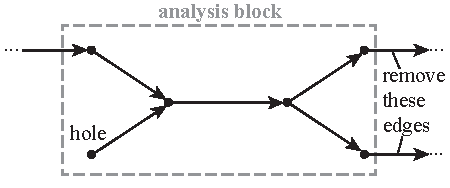
\includegraphics[width=3in]{images/analysis_block_hole}
        \end{center}
        \vspace{-20pt}
    \caption{Example variable node indicating a hole.}
    \label{f:hole}
    \end{figure}

    \item[Step 2: Collisions] 
        The second step is to detect collisions and to then disconnect enough connection edges so that the collisions are resolved. 
        The set of variable nodes which contain collisions is created as
    \begin{equation}
    S_\txt{nodes} = \{v \in V_M \st t_\txt{node}(v) = \txt{`variable'} \txt{ and } \txt{deg}^-(v) > \txt{deg}_u^-(v) \}.
    \end{equation}
    For each collision node we can construct a set contained the edges directed in. The set containing all of these sets is constructed as
    \begin{equation}
        S_\txt{edges} = \big \{ \{(x,y) \in E_M\} \ \big| \ y \in S_\txt{nodes} \big \}
    \end{equation}
    Let $J=\{1,2,\ldots,|S_\txt{edges}|\}$ be an indexing set for $S_\txt{edges}$ such that each $S_{\txt{edges},j}$ corresponds to a set in $S_\txt{edges}$ for $j \in J$. 
    An example collision is shown in Fig.~\ref{f:collision} to indicate the definition of $S_{\txt{edges},j}$. 
    We can assume that $J$ also indexes $S_\txt{nodes}$ because there is a one--to--one correspondence between the elements in $S_\txt{nodes}$ and the elements in $S_\txt{edges}$ (which are sets). 
    Then we may construct sets of edges as
    \begin{equation}
    B_j = \big \{e_k \in S_{\txt{edges},j} \st k \in \{1,2,\ldots,K\} \txt{ with } K \leq \txt{deg}_u^-(v_j) \big \}, \ j \in J,
    \end{equation}
        which means that each set $B_j$ is constructed from the set $S_{\txt{edges},j}$ by taking only as many edges as are allowed by the upper in--degree limit of $v_j$. 
        The construction of each $B_j$ corresponds to making a decision on which edges to include and which edges not to include. Then let
    \begin{equation}
    C_{F,2} = \{ e \in C_{F,1} \st e \in B_j \txt{ for some } j \in J\},
    \end{equation}
    \begin{equation}
    E_{F,2} = E_M \setminus (C_M \setminus C_{F,2})
    \end{equation}
    and
    \begin{equation}
    F_2 = (V_M,E_{F,2})
    \end{equation}
    \begin{figure}[htb!]
        \begin{center}
        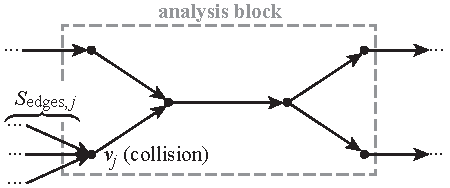
\includegraphics[width=3in]{images/analysis_block_collision}
        \end{center}
        \vspace{-20pt}
    \caption{Example variable node indicating a collision.}
    \label{f:collision}
    \end{figure}

    \item[Step 3: Finalize] 
        The third and final step is to prune the graph one last time
    \begin{equation}
        F = P_\txt{prune}(F_2),
    \end{equation}
        and $F = (V_F,E_F)$.
        The indices of the used analysis blocks can then be found as
    \begin{equation}
        I_F = \{ i \in I \st A_i \cap F \neq \emptyset \}
    \end{equation}
%       \begin{
%       \begin{equation}
%       I_F =  \{i \in I \ | \ \exists v \in V_{A_i} \txt{ such that }  t_\txt{node}(E_{F,2}^{-1}(v))=\txt{`model'} \txt{ and } \txt{deg}^+(v) > 0 \},
%       \end{equation}
%       where the degree is calculated with respect to $F_2$. 
%       This set excludes both the analysis blocks that were unused in the original MCG and those that became unused in step 1 or step 2.
%
%       The set of used global inputs is constructed as
%       \begin{equation}
%       V_{\txt{in},F} = \big\{v \in V_\txt{in} \ \big| \ |\{(x,y) \in E_{F,2}(v) \st y \in V_{A_i} \txt{ for } i \in I_F  \}| > 1 \big\},
%       \end{equation}
%       which requires that at least two edges directed out of the nodes in $V_{\txt{in},F}$ must be to the analysis blocks indexed by $I_F$.
%
%       Finally, the set of nodes and edges describing a fundamental problem graph is given by
%       \begin{equation}
%       V_F = V_{\txt{in},F} \cup V_\txt{out} \cup \left( \bigcup_{i \in I_F} V_{A_i} \right),
%       \end{equation}
%       \begin{equation}
%       C_{F} = \{ (x,y) \in C_{F,2} \st x,y \in V_F\},
%       \end{equation}
%       \begin{equation}
%       E_F = C_F \cup \left( \bigcup_{i \in I_F} E_{A_i} \right),
%       \end{equation}
%       \begin{equation}
%       F = (V_F,E_F).
%       \end{equation}

    \end{description}

This process will always provide an FPG if one exists. If an FPG does not exist, this process will reveal the limiting factors preventing a valid formulation.
\section{Example Problem}
	\label{s:example problem}
	This section presents an example problem to demonstrate the process of obtaining the FPG and the advantages of doing so. 
The example task is to create an FPG for the conceptual sizing of a single-aisle subsonic transport using a set of analysis tools with objectives including performance and gross weight for a required mission. 
	The full set of analysis codes available for use is provided in Table \ref{t:analysis codes}.
	\begin{table}[htbp]
	  \centering
	  \caption{Analysis codes for subsonic transport sizing}
		\begin{tabular}{cc}
		\toprule
		analysis code & description \\
		\midrule
		VSP   & parametric vehicle geometry \\
		PDCYL & wing and fuselage weight estimation \\
		NPSS  & engine sizing and performance \\
		VORLAX & aerodynamics using the vortex lattice method \\
		PMARC & aerodynamics using a low-order panel method \\
		WATE  & engine weight estimation \\
		FLOPSa & mission performance, \\
		  & engine sizing, and weight estimation \\
		FLOPSb & mission performance only \\
		\bottomrule
		\end{tabular}%
	  \label{t:analysis codes}%
	\end{table}%
	Each analysis code contributes individual disciplinary analysis capability, but the outputs of the codes are not mutually exclusive. 
	For example, VORLAX and PMARC are both aerodynamics codes that predict inviscid drag but with different levels of fidelity. 
	The Flight Optimization System (FLOPS) is included twice to represent two different configurations corresponding to different uses. 
	FLOPSa denotes FLOPS implemented to execute both mission performance and engine analysis, while FLOPSb indicates  FLOPS implemented to execute for only mission performance analysis. 
	This representation is useful for ``supercodes'' that are capable of being implemented in different ways and with different sets of inputs and outputs.
The enumeration of these analysis tools and objectives concludes step (A) in Sec.~\ref{ss:process}.

Step (B) is the production of the MCG.
	In this example, the MCG is formed using a consistant variable naming convention and then connecting all variables with the same name with connection edges. 
	Table \ref{t:ins and outs} presents the full list of variables in the leftmost column and indicates whether the variable is an input or an output of each analysis code. 
	Some variables, such as geometry and performance, represent groups of variables that are passed as arrays or other data structures due to their similarity. 
	This bundling of variables is not fundamental and does not limit the generality of this example; rather, it simplifies the presentation.
	\begin{table}[htb!]
	  \centering
	  \caption{Analysis code input and output description}
		\begin{tabular}{ccccccccc}
		\toprule
		variable & \multicolumn{8}{c}{analysis code} \\
		\midrule
			  & VSP   & PDCYL & NPSS  & VORLAX & PMARC & WATE  & FLOPSa & FLOPSb \\
		geometry & in    & in    &       & in    & in    & in    & in    & in \\
		number of engines &       &       & in    &       &       &       & in    & in \\
		mission &       &       &       &       &       &       & in    & in \\
		fuselage weight &       & out   &       &       &       &       & in    & in \\
		wing weight &       & out   &       &       &       &       & in    & in \\
		engine weight &       &       &       &       &       & out   & out   & in \\
		wetted area & out   &       &       &       &       &       & in    & in \\
		inviscid drag &       &       &       & out   & out   &       &       & in \\
		drag  &       &       & in    &       &       &       & out   & out \\
		engine performance &       &       & out   &       &       & in    & out   & in \\
		performance &       &       &       &       &       &       & out   & out \\
		total weight &       & in    &       &       &       &       & out   & out \\
		\bottomrule
		\end{tabular}
	  \label{t:ins and outs}
	\end{table}

	In this example, the MCG $M$ is formed in four steps:
	\begin{enumerate}
	\item An analysis block is created for each analysis code using the information in each column of Table \ref{t:ins and outs}. 
	Each analysis block is formed by first creating variable nodes for each input and adding directed edges into a single function node. An edge is directed from this function node into a second function node, which is then directed into variable nodes corresponding to each output. 
	A sample analysis block is shown for analysis code FLOPSa in Fig.~\ref{f:FLOPSb analysis block}.
	\begin{figure}[htb!]
	  \begin{center}
		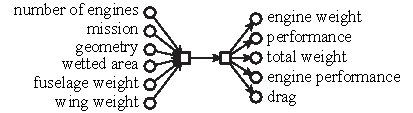
\includegraphics[width=2.75in]{images/FLOPSa_analysis_block}
	  \end{center}
	  \caption{Sample analysis block for analysis code FLOPSa using Table \ref{t:ins and outs}}
	\label{f:FLOPSb analysis block}
	\end{figure}

	\item Expression blocks are created to represent the objectives for performance and total weight.

	\item A variable nodes is created to represent the geometry variable as a input. Any inputs incorrectly omitted will be identified in step (D).

	\item Connection edges are created that connect each variable node to every other variable node representing variables with the same name. 
	The direction is determined by whether the variable node has an edge directed into or out of a function node, i.e. whether it is a local input or a local output.
	\end{enumerate}
	The resulting MCG is shown in Fig.~\ref{f:MCG holes}. 
	Cycles are shown as dashed lines. FPGs formed from this MCG may or may not retain these cycles.
	\begin{figure}[htb!]
	  \begin{center}
		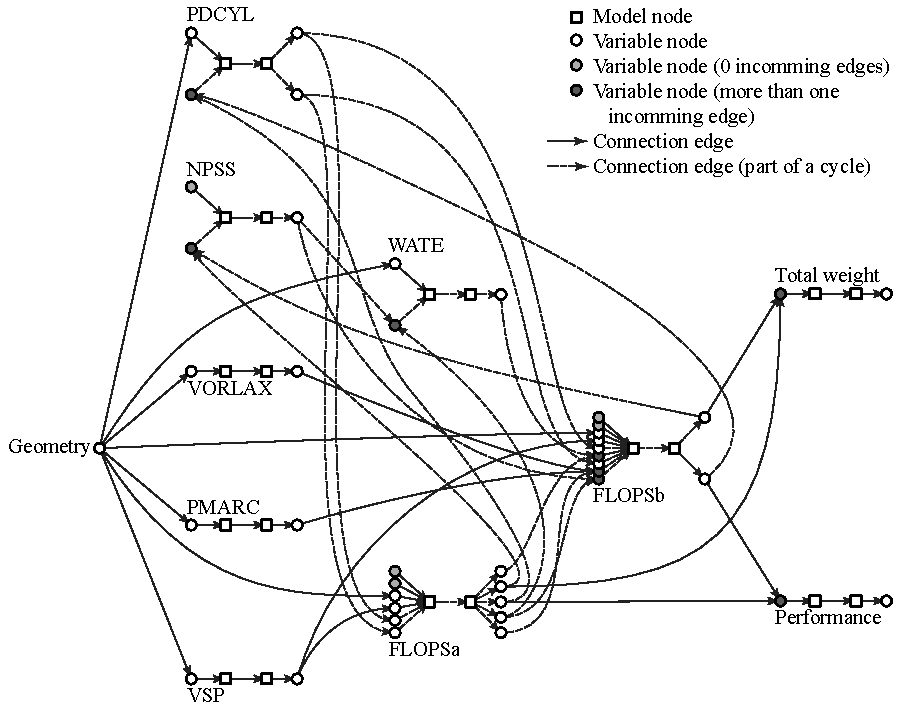
\includegraphics[width=6in]{images/MCG_edit_holes}
	  \end{center}
	  \caption{Maximal connectivity graph for the subsonic transport example problem}
	\label{f:MCG holes}
	\end{figure}

To implement step (C) in Sec.~\ref{ss:process}, the indegree of every variable node is set to unity to reflect a single fidelity analysis for which the design variables have not yet been selected.


%	As described in Sec.~\ref{ss:process}, the process of obtaining an FPG from the given MCG is expected to be an iterative process in which the user applies the algorithm to determine whether or not an FPG can be obtained, 
%	and then modifies the indegree limits or the MCG to obtain a satisfactory FPG.
%	For example, after determining the location of a hole, the user can change the indegree limit to make the node a design variable, or the user could change the MCG by adding a new analysis code such that the hole is resolved.
%
%	As presented in Sec.~\ref{s:building graphs}.\ref{ss:obtaining FPG}, the first step to obtaining an FPG is to detect holes. 
%	To begin, we set the lower indegree limit for every node to be unity. 

Step (D) now procededs by executing the FPG algorithm. An FPG cannot be obtained because the variable nodes representing the number of engines are holes for NPSS, FLOPSa, and FLOPSb, and the variable nodes representing the mission definition are holes for FLOPSa and FLOPSb. These holes propagated upstream and created holes in the objectives, thereby preventing a valid FPG.

Step (D)(a) begins to resolve this conflict by creating a input for the number of engines. In this example, the number of engines was not originally included as a input to demonstrate how the process responds to this error.
Step (D)(b) then reduces the lower and upper indegree limits for the variable node representing the mission definition to zero, implying that these nodes must be specified as design variables (see Table \ref{t:variable node classification}). The new MCG is shown in Fig.~\ref{f:MCG}.
	\begin{figure}[htb!]
	  \begin{center}
		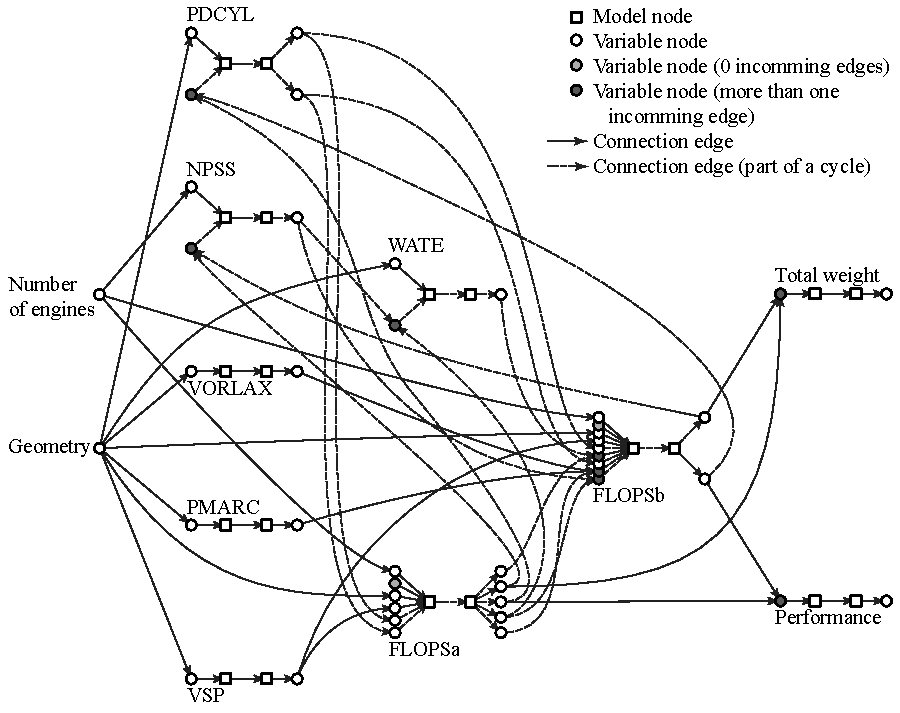
\includegraphics[width=6in]{images/MCG_edit}
	  \end{center}
	  \caption{The updated MCG with a new input.}
	\label{f:MCG}
	\end{figure}

	Although an FPG may now be obtained, this process has not provided a method to decide which edges to retain when resolving a collision, and these decisions will likely determine which analysis tools are included in the FPG. These decisions are left to the discretion of the designer in the context of the specific implementation. 
	However, the graph-based approach presented in this paper enables standard graph algorithms to be employed to automate these decisions based on considerations of metrics related to the graph or other data related to the analysis. 
	An example is a metric to obtain an FPG with the fewest possible number of cycles. 
In this example, the FPG with the fewest number cycles is shown in Fig.~\ref{f:FPG fewest cycles}, in which the edges belonging to a cycle are inticated by dashed lines. 
For this example problem, the cycles were detected using the implementation of Johnson's algorithm \cite{Johnson1975} in the Python package NetworkX. 
There are two cycles which arise from each local output from PDCYL being directed into FLOPSa and then back into PDCYL. 

	Similar alternatives would be to minimize the number of analysis blocks involved in cycles, counting multiplicity, or to minimize the length of the longest cycle (called the \emph{circumference} of the graph). It is beyond the scope of this work to explore efficient methods for finding the FPGs meeting these criteria. However, as discussed by Gabow\cite{Gabow1985}, graph algorithms typically scale well with the size of the graph. This suggests that the computation cost of finding an FPG should be small.
	\begin{figure}[htb!]
	  \begin{center}
		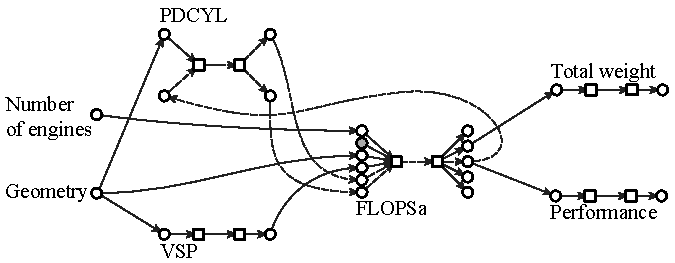
\includegraphics[width=4.5in]{images/FPG_edit_fewest_cycles}
	  \end{center}
	  \caption{FPG with the fewest number of cycles.}
	\label{f:FPG fewest cycles}
	\end{figure}

	Alternatively, it may be desirable to resolve collisions by choosing the higher fidelity analysis tools.
	One method to ensure that the edges directed from certain analysis blocks are those chosen to resolve conflicts is to use a ranking system. Each analysis block is assigned a value by the designer describing how desireable it is for this block to be present in the FPG. The connection edges directed out of each analysis block are then given a weight equal to the value assigned to the analysis block. Finally, each collision is resolved by selected the edges with the highest weights.
For the current example problem, consider the rankings for each analysis code given in Table \ref{t:rankings}.
	\begin{table}[htbp]
	  \centering
	  \caption{Example ranking of importance}
		\begin{tabular}{cc}
		\toprule
		analysis code & rank \\
		\midrule
		VSP   & 5 \\
		PDCYL & 5 \\
		NPSS  & 4 \\
		PMARC & 4 \\
		FLOPSb & 4 \\
		VORLAX & 3 \\
		WATE  & 3 \\
		FLOPSa & 2 \\
		\bottomrule
		\end{tabular}%
	  \label{t:rankings}%
	\end{table}%
	The resulting FPG has four cycles and is shown in Fig.~\ref{f:FPG highest rank}. 
%This graph has four cycles, which are enumerated in Table \ref{t:cycles}.
	\begin{figure}[htb!]
	  \begin{center}
		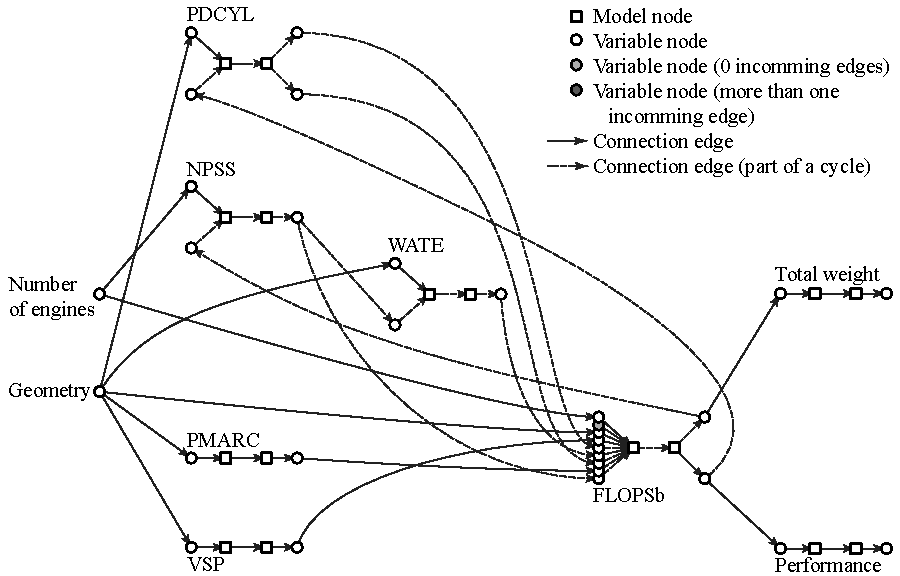
\includegraphics[width=6in]{images/FPG_edit_ranking}
	  \end{center}
	  \caption{FPG obtained using the ranking system.}
	\label{f:FPG highest rank}
	\end{figure}
%	\begin{table}[htbp]
%	  \centering
%	  \caption{Cycles for the FPG obtained using ranking}
%		\begin{tabular}{ccccccc}
%		\toprule
%		output/input & analysis code & output/input & analysis code & output/input & analysis code & output/input \\
%		\midrule
%		engine weight & FLOPSb & drag  & NPSS  & engine performance & WATE  & engine weight \\
%		engine performance & FLOPSb & drag  & NPSS  & engine performance &       &  \\
%		fuselage weight & FLOPSb & total weight & PDCYL & fuselage weight &       &  \\
%		wing weight & FLOBSb & total weight & PDCYL & wing weight &       &  \\
%		\bottomrule
%		\end{tabular}%
%	  \label{t:cycles}
%	\end{table}%

	Finally, consider a case in which 
the inviscid drag input into FLOPSb is a multi-fidelity input, meaning that 
 multiple analysis codes calculate the same variable. 
	This multi-fidelity formulation is implemented by setting the upper indegree limit for this node as two and then repreating the (automated) process. 
	In this case, both VORLAX and PMARC are retained, resulting in an FPG that omits only FLOPSa.


\section*{Conclusions}
In this paper, we have presented an approach for describing  MDAO problems with 
with a graph based syntax.  Our graph description shares 
similarities to other approaches such as REMS, FDT, DSM, and XDSM, but 
it provides new constructs tailored to applications in early phases of the design 
process where a problem formulation has not yet been fully formed.   
In particular, we introduce the concepts of the Maximal Connectivity Graph (MCG) 
and the Fundamental Problem Graph (FPG).  

The MCG addresses the question, ``Given a set of analysis tools and design objectives, what are all 
of the potential problem formulations that could exist to solve a design problem?''  
The MCG provides a structured formalism to reduce the, potentially very large, 
set of valid combinations of analysis tools to a single subset and to identify
conflicts that could prevent a valid problem formulation.
Conflicts can originate from two sources: holes and collisisons. A hole 
corresponds to a variable that is not calculated by any analysis block in the 
MCG but is needed by other blocks. To create a valid problem formulation, all 
holes must be ``filled'' either by selecting the corresponding variable as a 
design variable, or by introducing additional analysis tools to compute the variable.  
A collision happens when two or more analysis tools compute values for the same variable.  
To create a valid problem formulation, all collisions must be resolved either by 
removing redundant analysis tools or by explicitly allowing the redundencies to remain 
in the form of a multifidelity problem. For the latter case, a special solution 
method will need to be employed to manage the multifidelity situation and decide 
when to execute the different analysis tools. Resolving collisions and filling 
holes in an MCG both require choices by the designer to shape the overall
MDAO problem to meet the needs of the problem he/she is trying to solve. 

The FPG represents the problem as an engineer would describe it: ``Given a specific set of tools, 
with a set of design vairables, find design that best meets a given objective
within the given constraints.'' Although an FPG uniquely defines a single MDAO problem, 
there is not necessarily a unique FPG for any given MCG. In Section 
\ref{s:building graphs} we provide an algorithm 
that reduces an MCG, via the resolution of conflicts in the graph, down to an FPG. 
How one goes about resolving the conflicts will determine which particular FPG is reached. 
One benefit of using graph theory is the standard techniques, such as cycle 
detection, which can be used to inform the user's decisions and make the process of conflict 
resolution much easier. 

In Section \ref{s:example problem}, we provide an example of 
formulating different FPGs from an MCG for a commercial aircraft design problem. This problem includes 8 
analysis tools and approximately 20 variables. Despite this relatively modest size, 
the MCG is rich enough to provide for a number of different valid FPGs. This demonstrates
the inherant value of the MCG to the design process by providing a mechanism for selecting 
an FPG based on important factors such as available design cycle time, consideration of 
coupling effects, or desired fidelity. Even after downselecting to a single FPG, the 
MCG itself still remains a useful tool. No real design problem is static, and will always
evolve throughout the design process. New tools may be introduced to account for previously 
unexpected effects and new constraints or objectives can be introduced. When this occurs, 
the MCG provides the opportunity to account for these changes by starting over with the 
algorithm from Section \ref{s:building graphs} to downselect to the most effective new FPG. 
While it is possible that this new FPG will be very similar to the previous one, 
it is also very possible that it will be different in significant ways. 
By repeating downselection algorithm from the MCG you allow for any new interdisciplinary couplings and  
information conflicts to play a role in selecting the most appropriate FPG. 

Once a desired FPG is identified, the driver node and driven edge described in the paper can be 
leveraged to formulate a Problem Solution Graph (PSG). This graph includes all of the 
same information from the FPG while additionally describing the particular MDAO 
solution architecture, e.g. MDF, IDF, BLISS, ATC, that will be used to solve the problem.  
Many possible PSGs could be formulated to solve a problem corresponding to a 
specified FPG. The application of the syntax to PSGs has not been illustrated in the paper, 
but the basic concept of applying multiple solution strategies to a given problem 
formulation has been well established by a number of MDAO architecture 
benchmarking efforts. Furthermore the validity of applying 
graph syntax to the description of specific problem solutions has been demonstrated 
by XDSM. 

For simple problems with few analysis tools and variables, the formulation of a 
valid problem description is straightforward.  However, MDAO problems continue to 
grow in scale and complexity. As the numbers of analysis tools and variables have 
increased, it has become increasingly challenging and time consuming for engineering 
teams to determine how the multiple analysis tools can be interconnected to produce 
valid problem formulations. Large complex problems also present signficant challenges
as the design process evolves requiring the integration high-fidelity 
analysis tools into an existing model. The graph syntax presented in this paper 
is intended to offer value in this context of increasing problem complexity by 
providing a formal approach to identify and resolve data conflicts in a set of interconnected
analysis tools and to help arrange those tools into an effective and efficient system model
where MDAO tools and techniques can be quickly and easily applied.  




\bibliography{library}
\end{document}
